\documentclass[11pt,a4paper,french,twoside]{PMCours}
\usepackage{hyperref}
\frenchbsetup{StandardLists=true}
\newcounter{activite}
\newcommand{\activite}{\subsubsection*{Activité~\refstepcounter{activite}\theactivite}}

\begin{document}
\TitreISN{Classe de Terminale}{Année 2021--2022}
{Numérique et Sciences Informatiques}{Entrainement à l'\'Epreuve de Spécialité - Sujet 1 - 3h30}
\ \medskip\\
{\large Chaque candidat traitera trois exercices au choix parmi les quatre proposés, chaque exercice étant noté sur sept points.\medskip\\
L'usage de tout document, calculatrice, etc... est interdit. \medskip\\
Les élèves rendront de manière impérative brouillons et sujet en même temps que leur composition.}

%\tableofcontents

%
%
%
%
\newpage\noindent
\section*{Exercice 1}
\emph{Cet exercice porte sur le maniement de listes Python et sur des questions liées à l'algorithmique.}\medskip\\
On se donne l'algorithme suivant dans lequel \code{t} est un tableau dont les éléments sont indexés de manière classique, c'est à dire à partir de $0$.\ \\
\begin{Python}
Fonction myst(t)
n = longueur(t)
Pour i de 0 à n-2
	Pour j de 0 à n-2
		Si t[j] >t [j+1]
		Alors
			échanger t[j] et t[j+1]
			#afficher (i,j,t)
renvoyer(t)
\end{Python}
\begin{enumerate}
\item On exécute les commandes suivantes en console Python :\medskip\\
. \hskip -1cm \begin{tabular}{p{5cm}p{5cm}p{5cm}}
\begin{Python}
code 1
a=5
b=7
b=a
a=b
print(a,b)
\end{Python} 
&
\begin{Python}
code 2
a=5
b=7
c=a
a=b
b=c
print(a,b)
\end{Python} 
&
\begin{Python}
code 3
a=5
b=7
a,b=b,a
print(a,b)
\end{Python} 
\end{tabular}\\
Donner, pour les trois codes, le résultat de l'affichage.
\item Implémenter la fonction \code{myst} en langage Python.
\item Pour observer le déroulement de l'algorithme, on décommente la ligne 7 et on 
l'exécute avec \code{t=[13, -5, 7,2, -8, 15, 1, -9, 9]}.\\
On obtient alors :
\begin{multicols}{2}
\begin{tabular}{lcl}
 init & :  & [13, -5, 7,2, -8, 15, 1, -9, 9]\\
0,& 0,& [-5, 13, 7, 2, -8, 15, 1, -9, 9]\\
0,& 1,& [-5, 7, 13, 2, -8, 15, 1, -9, 9]\\
0,& 2,& [-5, 7, 2, 13, -8, 15, 1, -9, 9]\\
0,& 3,& [-5, 7, 2, -8, 13, 15, 1, -9, 9]\\
0,& 5,& [-5, 7, 2, -8, 13, 1, 15, -9, 9]\\
0,& 6,& [-5, 7, 2, -8, 13, 1, -9, 15, 9]\\
0,& 7,& [-5, 7, 2, -8, 13, 1, -9, 9, 15]\\
1,& 1,& [-5, 2, 7, -8, 13, 1, -9, 9, 15]\\
1,& 2,& [-5, 2, -8, 7, 13, 1, -9, 9, 15]\\
1,& 4,& [-5, 2, -8, 7, 1, 13, -9, 9, 15]\\
1,& 5,& [-5, 2, -8, 7, 1, -9, 13, 9, 15]\\
1,& 6,& [-5, 2, -8, 7, 1, -9, 9, 13, 15]\\
\end{tabular}
\begin{tabular}{lcl}
2,& 1,& [-5, -8, 2, 7, 1, -9, 9, 13, 15]\\
2,& 3,& [-5, -8, 2, 1, 7, -9, 9, 13, 15]\\
2,& 4,& [-5, -8, 2, 1, -9, 7, 9, 13, 15]\\
3,& 0,& [-8, -5, 2, 1, -9, 7, 9, 13, 15]\\
3,& 2,& [-8, -5, 1, 2, -9, 7, 9, 13, 15]\\
3,& 3,& [-8, -5, 1, -9, 2, 7, 9, 13, 15]\\
4,& 2,& [-8, -5, -9, 1, 2, 7, 9, 13, 15]\\
5,& 1,& [-8, -9, -5, 1, 2, 7, 9, 13, 15]\\
6,& 0,& [-9, -8, -5, 1, 2, 7, 9, 13, 15]\\
\end{tabular}
\end{multicols}
Et le résultat renvoyé est \code{[-9, -8, -5, 1, 2, 7, 9, 13, 15]}
\begin{enumerate}
\item Que fait cette fonction ? (Décrire uniquement le résultat final). 
\item Donner la valeur de \code{n}. Quels sont les domaines parcourus par \code{i} et \code{j} ? 
\item Est-ce que la fonction génère un affichage pour chaque valeur du couple \code{(i,j)} ? Pourquoi ? 
\item Donner \code{t} à la fin du traitement correspondant à \code{(i=0,j=5)}, à \code{(i=2,j=5)} et à \code{(i=3,j=1)}.
\end{enumerate}
Sur l'exemple précédent, on observe que \code{13} ''remonte'' comme une bulle à la surface jusqu'à ce qu'il rencontre un élément plus grand que lui (qui est \code{15}) et c'est alors cet élément qui remonte, etc.. \\
A la fin du passage en boucle pour \code{i=0}, on observe que \code{15} est ''à sa place'', etc... 
\item On prend maintenant \code{t=[11,9,3,15,-9]} et on lui applique le programme. 
\begin{enumerate}
\item Donner la valeur de \code{n}. Quels sont les domaines parcourus par \code{i} et \code{j} ? 
\item Donner les diffférentes valeurs que \code{t} prendra (on ne demande pas les \code{i} et \code{j} correspondants) et en particulier, donner la valeur finale de \code{t}
\end{enumerate}
\item Que peut-on dire du tableau \code{t} quand on a terminé l'exécution de la première boucle pour un \code{i} fixé dans $\{0,\cdots,n-2\}$ ? 
\item 
\begin{enumerate}
\item On veut estimer le coût de l'algorithme en installant un compteur \code{c} comptabilisant le nombre exact d'opérations effectuées. \\
On compte une opération pour chaque test et deux opérations pour chaque échange.\\
Recopier l'algorithme (ou le code Python) en rajoutant les commandes concernant \code{c}.
\item En ayant procédé ainsi, on teste ce programme sur des listes aléatoires de longueur \code{n} et on obtient le tableau suivant :\medskip\\
\begin{tabular}{|p{2cm}|p{2cm}|p{2cm}|p{2cm}|p{2.5cm}|}\hline
n&$10$&$10^2$&$10^3$&$10^4$\\ \hline
c&125&14\,899&1\,475\,589&150\,358\,643\\ \hline
c&117&14\,745&1\,492\,811&150\,358\,643\\ \hline
\end{tabular}\medskip\\
Le coût d'exécution du programme semble-t-il être linéaire (c'est à dire proportionnel à \code{n}), quadratique (c'est à dire proportionnel à \code{n}$^2$) ?
\item Confimer cela par une brève remarque sur la structure du programme. 
\item Existe-t-il des cas de \code{t} pour lesquels on fera un minimum d'opérations ? Un maximum d'opérations ? Justifier.
\end{enumerate} 
\item Peut-on facilement modifier le programme pour en faire un tri dans l'ordre décroissant ? Si oui, indiquer cette modification.
\item Proposer l'implémentation en Python d'un autre algorithme de tri parmi ceux au programme de NSI.  
\end{enumerate} 

\newpage\noindent

\section*{Exercice 2}
\emph{Cet exercice porte sur les bases de données relationnelles et le langage SQL}\medskip\\

L'énoncé de cet exercice utilise les mots du langage SQL suivant :
\begin{verbatim}
SELECT, FROM, WHERE, JOIN, INSERT INTO, VALUES, ORDER BY, DISTINCT, COUNT
\end{verbatim}

On s'intéresse au parc informatique d'un lycée, constitué d'ordinateurs, d'imprimantes, de vidéoprojecteurs et de TNI (Tableau Numérique Interactif). Tous les ordinateurs et toutes les imprimantes sont connectés au réseau de l'établissement. Chaque salle de cours est identifiée par un numéro unique et contient : 
\begin{itemize}
\item un ou plusieurs ordinateurs reliés au réseau,
\item aucun ou un seul vidéoprojecteur,
\item s'il y a un vidéoprojecteur, aucun ou un seul TNI,
\item une ou plusieurs imprimantes réseau.
\end{itemize}

Un ordinateur peut être connecté via le réseau à une ou plusieurs imprimantes (situées éventuellement dans une ou plusieurs salles) et à un vidéoprojecteur avec TNI ou non.
Les ordinateurs et les imprimantes possèdent un nom unique sur le réseau de l'établissement.
Les vidéoprojecteurs ne sont pas connectés au réseau, ils ne possèdent pas de nom unique. Ils sont donc identifiés par le numéro de la salle où ils sont installés.
Tous ces matériels sont gérés à l'aide d'une base de données relationnelle, qui comprend 3 relations (ou tables) nommées : \verb'Ordinateur', \verb'Videoprojecteur', \verb'Imprimante'.

On donne ci-dessous le schéma relationnel de la relation  \verb'Ordinateur' : 

\verb'Ordinateur' (\underline{nom\_ordi} : String, \verb'salle' : String, \verb'marque_ordi' : String, \verb'modele_ordi' : String, \verb'annee' : Int, \verb'video' : Boolean)

Par convention, la clé primaire est soulignée  et les éventuelles clés étrangères sont repérées par le symbole \verb'#'.

On affiche ci-dessous les 5 premières lignes de la relation \verb'Ordinateur' :
\begin{figure}[h]
\begin{center}
\begin{tabular}[c]{|c|c|c|c|c|c|}\hline
\verb'nom_ordi' & \verb'salle' & \verb'marque_ordi' & \verb'modele_ordi' & \verb'annee' & \verb'video'\\\hline
Gen-24 & 012 & HP & compaq pro 6300 & 2012 & true\\\hline
Tech-62 & 114 & Lenovo & p300 & 2015 & true\\\hline
Gen-132 & 223 & Dell & Inspiron Compact & 2019 & true\\\hline
Gen-133 & 223 & Dell & Inspiron Compact & 2019 & false\\\hline
Gen-134 & 223 & Dell & Inspiron Compact & 2019 & false\\\hline
\end{tabular}
\end{center}
\caption{Extrait de la relation \textbf{Ordinateur}}
\end{figure}

On distingue deux types d'ordinateur :
\begin{itemize}
\item les ordinateurs multimédias pour les logiciels généraux avec un nom commençant par le groupe de lettres Gen ;
\item les ordinateurs techniques pour les logiciels qui demandent plus de ressources avec un nom commençant par le groupe de lettres Tech.
\end{itemize}
Ce groupe de lettres est suivi d'un tiret et du numéro unique de l'ordinateur pour chaque type.




\begin{enumerate}

\item On exécute sur un système de gestion de base de données la requête SQL :
\begin{verbatim}
SELECT salle, marque_ordi FROM Ordinateur
\end{verbatim}
Quel résultat produit cette requête, sur l'extrait de la relation \verb'Ordinateur' donné ci-dessus ?


\item Soit la requête SQL :
\begin{verbatim}
SELECT salle, marque_ordi FROM Ordinateur WHERE video = true
\end{verbatim}
Quel résultat produit cette requête, sur l'extrait de la relation \verb'Ordinateur' donné ci-dessus ?


\item Ecrire une requête SQL donnant tous les attributs des ordinateurs correspondant aux années supérieures ou égales à 2017 ordonnées par dates croissantes.


\item Pour quelle raison l'attribut \verb'salle' ne peut-il pas être une clé primaire pour la relation \verb'Ordinateur' ?



\end{enumerate}


\begin{figure}[h]
\begin{center}
\begin{tabular}[c]{|c|c|c|c|c|}\hline
\verb'nom_imprimante' & \verb'marque_imp' & \verb'modele_imp' & \verb'salle' & \verb'nom_ordi'  \\\hline
imp-BTS-NB & HP & Laserjet pro M15w & 114 & Tech-62  \\\hline
imp-BTS-Couleur & Canon & Megatank Pixma G5050 & 114 & Tech-62  \\\hline
imp-salle-info1 & Brother & 2360DN & 223 & Gen-132  \\\hline
imp-salle-info1 & Brother & 2360DN & 223 & Gen-133  \\\hline
imp-salle-info1 & Brother & 2360DN & 223 & Gen-134  \\\hline
\end{tabular}
\end{center}
\caption{Extrait de la relation \textbf{Imprimante}}
\end{figure}

\begin{enumerate}
\setcounter{enumi}{4}

\item On prend \verb'(nom_imprimante, nom_ordi)' comme clé primaire de la relation \verb'Imprimante' écrite ci-dessus. Ecrire le schéma relationnel de cette relation.


\end{enumerate}


\begin{figure}[h]
\begin{center}
\begin{tabular}[c]{|c|c|c|c|}\hline
\verb'salle' & \verb'marque_video' & \verb'modele_video' & \verb'tni'  \\\hline
012 & Epson & xb27 & true  \\\hline
114 & Sanyo & PLV-Z3 & false  \\\hline
223 & Optoma & HD143X & false  \\\hline
225 & Optoma & HD143X & true  \\\hline
\end{tabular}
\end{center}
\caption{Extrait de la relation \textbf{Videoprojecteur}}
\end{figure}

\begin{enumerate}
\setcounter{enumi}{5}

\item Ecrire une requête SQL pour ajouter à la relation \verb'Videoprojecteur', écrite ci-dessus, le vidéoprojecteur nouvellement installé en salle 315 de marque NEC, modèle ME402X et non relié à un TNI.

\item Ecrire une requête SQL qui affiche le nom des différents modèles de vidéoprojecteurs installés dans le lycée, de marque Epson, sans répétition.

\item Ecrire une requête SQL permettant de récupérer les attributs \verb'salle', \verb'nom_ordi', \verb'marque_video' des ordinateurs connectés à un vidéoprojecteur équipé d'un TNI.

\item Ecrire une requête SQL qui renvoie le nombre d'ordinateurs situés dans des salles où il y a un vidéoprojecteur de marque Optema.

\item Ecrire une requête SQL qui renvoie le nom des salles où sont installés dans une même pièce un ordinateur de marque Dell, une imprimante de marque HP et un vidéoprojecteur de marque Epson.


\end{enumerate}


\newpage\noindent
\section*{Exercice 3}
\emph{Cet exercice traite principalement le thème \og{} algorithmique
langages et programmation\fg{}.}\medskip\\

L'objectif de cet exercice est de permettre, dans le service des urgences
d'un hôpital, la prise en compte de la gravité des cas dans la gestion
de l'ordre de passage des patients.

\medskip
On choisit de représenter la file d'attente par un tableau (type \code{list})
dont les éléments sont de objets définis par la classe suivante :
\begin{Python}
class Patient:
    def __init__(self, nom, prenom, age, gravite):
        self.nom=nom
        self.prenom=prenom
        self.age=age
        self.gravite=gravite
\end{Python}
Chaque patient est donc défini par son nom, son prénom, son âge (en années)
et la gravité de son cas (qui est un entier de $1$ à $10$, $1$ correspondant
aux cas sans urgence et 10 aux cas d'urgence vitale).

\begin{enumerate}
    \item On exécute une à une les instructions suivantes :
\begin{Python}
attente=[]
attente.append(Patient("Martin","Abel",35,1))
attente.append(Patient("Dupond","Béatrice",42,5))
attente.append(Patient("Laurent","Charles",60,2))
\end{Python}
\begin{enumerate}
    \item Quel est le résultat de l'exécution de \code{L[1].age} ?
    \item Quel est le résultat de l'exécution de \code{L[2].prenom[1]} ?
    \item Quelle commande exécuter pour passer la gravité de Béatrice à $7$ ?
\end{enumerate}    
    \item On considère la fonction suivante:
\begin{Python}
def mystere(attente):
    A=0
    for k in range(len(attente)):
        if attente[k].age>A:
            A=attente[k].age
    return A
\end{Python}
    Pour une liste \code{attente} d'objets de classe \code{Patient} quelconque,
    que fait cette fonction ?
    \item Écrire (en s'inspirant de la question précédente) une fonction \code{cas\_critique(attente)} qui détermine
    le cas le plus grave ou, s'il y a égalité, le plus jeune.
    Cette fonction doit retourner le rang du patient en question dans la liste 
    \code{attente}.
    \item On exécute une à une les instructions suivantes :
\begin{Python}
attente=[]
attente.append(Patient("Martin","Abel",35,1))
attente.append(Patient("Dupond","Béatrice",42,5))
attente[0]=attente[1]
attente[1]=attente[0]
\end{Python}
    Choisissez une réponse parmi les cinq suivantes :
    \begin{enumerate}
        \item La liste \code{attente} contient deux fois le patient Martin. 
        \item La liste \code{attente} contient deux fois la patiente Dupond. 
        \item La liste \code{attente} est inchangée. 
        \item Les patients Martin et Dupond ont échangé leur place dans la liste \code{attente}. 
        \item Une erreur se produit à l'exécution. 
    \end{enumerate}
    \item On exécute une à une les instructions suivantes :
\begin{Python}
attente=[]
attente.append(Patient("Martin","Abel",35,1))
attente.append(Patient("Dupond","Béatrice",42,5))
x=attente[1]
attente[1]=attente[0]
attente[0]=x
\end{Python}
    Choisissez une réponse parmi les cinq suivantes :
    \begin{enumerate}
        \item La liste \code{attente} contient deux fois le patient Martin. 
        \item La liste \code{attente} contient deux fois la patiente Dupond. 
        \item La liste \code{attente} est inchangée. 
        \item Les patients Martin et Dupond ont échangé leur place dans la liste \code{attente}. 
        \item Une erreur se produit à l'exécution. 
    \end{enumerate}
    \item Écrire une fonction \code{doubler(attente,k)}, qui compare les patients
    correspondants aux index $k-1$ et $k$ et les échange éventuellement pour que
    le cas le plus grave (le plus âgé, s'ils ont la même gravité) soit en position $k-1$.
    \item Écrire une fonction \code{suivant(attente)}, qui appliqué la fontion 
    \code{doubler} à toute la file d'attente, en commençant par les plus petits 
    index. Puis renvoie le premier patient en le retirant la liste.
    \item On souhaite modifier la fonction \code{doubler(attente,k)} pour qu'elle
    déplace le patient d'index $k$ vers la gauche et ce tant que le total de 
    gravité des patients qu'il dépasse est strictement inférieur 
    à sa propre gravité. (Un patient de gravité $5$ pourra dépasser les trois 
    patients qui le précèdent si leurs gravités sont $1$, $2$, $1$, 
    mais il s'arrêtera là car $1+2+1=4<5$.)
    
    Compléter le code suivant :
\begin{Python}
def doubler(attente,k):
    g=attente[k].gravite
    i=k-1
    S=0
    while ____ and _______________:
        S=S+attente[i].gravite
        attente[i],attente[i+1]=_________________________
        i=___
\end{Python}
\end{enumerate}


\newpage\noindent

\section*{Exercice 4}
\emph{Cet exercice porte principalement sur la programmation orientée objet, les listes chaînées et la récursivité.}\medskip\\
Dans cet exercice, on modélise un train au moyen d'une liste chainée. 
\begin{Python}
class Wagon : 
	def __init__(self,b,m,s) : 
		self.motrice=b
		if self.motrice :
			self.puissance=5000
		else : 
			self.puissance=0
		if  _________
			self.charge = m
		else :
		    _________
		self.suivant=s
\end{Python}
La classe \code{Wagon} a les attributs suivants : 
\begin{itemize}
\item \code{motrice} de type \code{bool}, valant \code{True} si le train est une motrice et \code{False} sinon.
\item \code{puissance} de type \code{int}, valant \code{5000} si le train est une motrice et \code{0} sinon.
\item \code{charge} de type \code{int}, représentant la charge transportée par le wagon.
\item \code{suivant} qui est une instance de la classe \code{Wagon}, représentant le wagon qui situé après lui dans le train, ou valant \code{None} si le wagon est le dernier. 
\end{itemize}
\begin{enumerate}
\item \begin{enumerate}
\item Recopier et compléter sur votre copie les lignes \code {8} et \code{11} du constructeur de la classe Wagon afin que la \code{charge} soit égale à \code{m} si le wagon est un wagon de transport et \code{0} sinon.
\item On considère le convoi suivant dans lequel : 
\begin{itemize}
\item un wagon de transport est représenté par un rectangle portant le nom de la variable et sa charge;
\item une motrice est représentée par un rond portant le nom de la variable.
\end{itemize}
Le convoi est représenté avec la {\bf tête à droite} et la {\bf queue à gauche} : \medskip\\
\centerline{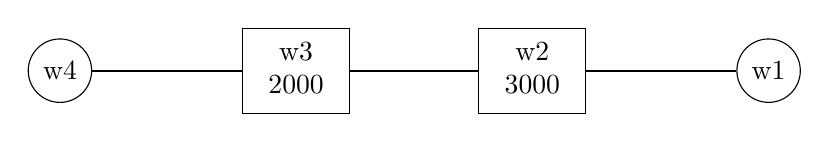
\begin{tikzpicture}[xscale=1,yscale=1]
% Styles (MODIFIABLES)
\tikzstyle{fleche}=[-,>=latex,thick]
\tikzstyle{wagon}=[rectangle,draw]
\tikzstyle{motrice}=[circle,draw]
% Dimensions (MODIFIABLES)
\def\DistanceInterNiveaux{3}
\def\DistanceInterFeuilles{2}
% Dimensions calculées (NON MODIFIABLES)
\def\NiveauA{(-0)*\DistanceInterNiveaux}
\def\InterFeuilles{(.75)*\DistanceInterFeuilles}
% Noeuds (MODIFIABLES : Styles et Coefficients d'InterFeuilles)
\node[motrice] (C1) at ({(6)*\InterFeuilles},{\NiveauA}) {w1};
\node[wagon] (C2) at ({(4)*\InterFeuilles},{\NiveauA}) {\begin{tabular}{c}w2\\3000 \end{tabular}};
\node[wagon] (C3) at ({(2)*\InterFeuilles},{\NiveauA}) {\begin{tabular}{c}w3\\2000 \end{tabular}};
\node[motrice] (C4) at ({(0)*\InterFeuilles},{\NiveauA}) {w4};
% Arcs (MODIFIABLES : Styles)
\draw[fleche] (C2)--(C1);
\draw[fleche] (C3)--(C2);
\draw[fleche] (C4)--(C3);
\end{tikzpicture}}
\\
Et par exemple, {\bf si on suppose que \code{w3} a été créée}, on peut créer \code{w2} au moyen de la commande \code{w2=Wagon(False,3000,w3)} car ce wagon n'est pas une motrice, a une charge de \code{3000} et a pour wagon suivant \code{w3}.\medskip\\
{\bf On suppose initialement qu'aucune variable n'a été créée.} \\
Donner les commandes Python permettant de créer le convoi ci-dessus.
\item Donner alors les résultats des appels suivants : \\
- \code{w1.motrice}\\
- \code{w1.suivant.charge}\\
- \code{w2.suivant.suivant.puissance}\\
- \code{w2.suivant.suivant.suivant}\\
- \code{w3.suivant.suivant.charge}
\item En reprenant les mêmes conventions, représenter sous forme de schéma le convoi construit au moyen des commandes suivantes :
\begin{Python}
D = Wagon(False,2000,None)
C = Wagon(True,0,None)
A = Wagon(True,0,C)
B = Wagon(False,5000,None)
D.suivant = B
C.suivant = D
\end{Python}
\end{enumerate}
\item Pour gérer plus efficacement cette situation, on considère maintenant une classe \code{Train} donnée par : 
\begin{Python}
class Train : 
	def __init__(self,w) : 
		self.tete = w
		
	def ajout_tete(self,w) : 
		'''ajoute le wagon w en tête de train'''
		w.suivant=self.tete
		self.tete=w
		
	def queue(self) : 
		'''renvoie le dernier wagon du train'''
		a=self.tete
		while a.suivant is not None :
			a=a.suivant
		return a
\end{Python}	 	 



\end{enumerate}
\end{document}





\newpage
\section*{Exercice 1}
\emph{Cet exercice porte sur les piles et leur implémentation en langage Python.}\\

\includegraphics[width=18cm]{images/page1.png}

\ \\

\includegraphics[width=17.5cm]{images/page2.png}

\includegraphics[width=18cm]{images/page3.png}
\includegraphics[width=17cm]{images/page4.png}



%
%
%
%
\newpage
\section*{Exercice 2}
\emph{Cet exercice porte sur les graphes et leur implémentation en langage Python.}\\
On rappelle que les graphes peuvent être représentés par des matrices d'adjacences ou par des dictionnaires. \medskip\\
\begin{tabular}{p{5cm}p{4cm}p{9.3cm}}
Par exemple, le graphe &correspond à la matrice&et au dictionnaire \\\\\
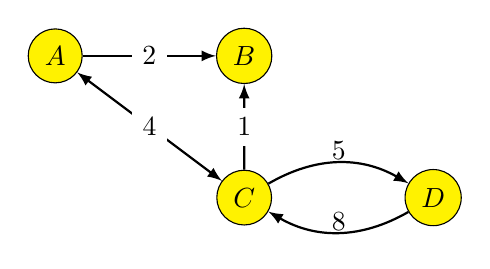
\begin{tikzpicture}[xscale=.6,yscale=.6]
% Styles (MODIFIABLES)
\tikzstyle{fleche}=[<->,>=latex,thick]
\tikzstyle{sfleche}=[->,>=latex,thick]
\tikzstyle{noeud}=[fill=yellow,circle,draw]
\tikzstyle{feuille}=[fill=orange,circle,draw]
\tikzstyle{etiquette}=[midway,fill=white,draw=white]
\tikzstyle{etiquette2}=[rectangle,fill=white,draw=white]
% Dimensions (MODIFIABLES)
\def\DistanceInterNiveaux{3}
\def\DistanceInterFeuilles{2}
% Dimensions calculées (NON MODIFIABLES)
\def\NiveauA{(-0)*\DistanceInterNiveaux}
\def\NiveauB{(-1)*\DistanceInterNiveaux}
\def\InterFeuilles{(1)*\DistanceInterFeuilles}
% Noeuds (MODIFIABLES : Styles et Coefficients d'InterFeuilles)
\node[noeud] (A) at ({(0)*\InterFeuilles},{\NiveauA}) {$A$};
\node[noeud] (B) at ({(2)*\InterFeuilles},{\NiveauA}) {$B$};
\node[noeud] (C) at ({(2)*\InterFeuilles},{\NiveauB}) {$C$};
\node[noeud] (D) at ({(4)*\InterFeuilles},{\NiveauB}) {$D$};
\node[etiquette2] (e1) at (6,-2) {5};
\node[etiquette2] (e1) at (6,-3.5) {8};
% Arcs (MODIFIABLES : Styles)
\draw[sfleche] (A)--(B) node[etiquette] {$2$} ;
\draw[fleche] (A)--(C) node[etiquette] {$4$} ;
\draw[sfleche] (C)--(B) node[etiquette] {$1$};
\draw[sfleche] (C) to [bend left] (D);
\draw[sfleche] (D) to [bend left] (C);
\end{tikzpicture}
&.\vskip -3cm$T=\left(\begin{array}{cccc}
0&2&4&0\medskip\\
0&0&0&0\medskip\\
4&1&0&5\medskip\\
0&0&8&0\medskip\\
\end{array}\right)  $
&
.\vskip -3cm \begin{Python}
di={'A':{'B':2,'C':4}, 
'B':{}, 
'C':{'A':4,'B':1,'D':5}, 
'D':{'C',8}}
\end{Python}

\end{tabular}
\subsection*{Question 1}
\begin{enumerate}
\item Donner la matrice d'adjacence et le dictionnaire correspondant au graphe : \medskip\\
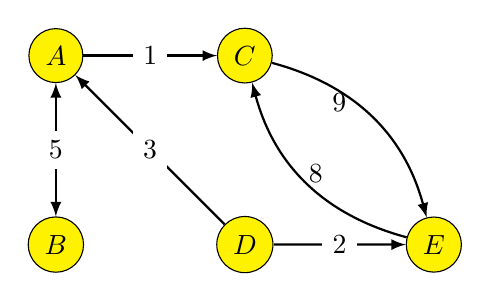
\begin{tikzpicture}[xscale=.6,yscale=.6]
% Styles (MODIFIABLES)
\tikzstyle{fleche}=[<->,>=latex,thick]
\tikzstyle{sfleche}=[->,>=latex,thick]
\tikzstyle{noeud}=[fill=yellow,circle,draw]
\tikzstyle{feuille}=[fill=orange,circle,draw]
\tikzstyle{etiquette}=[midway,fill=white,draw=white]
\tikzstyle{etiquette2}=[rectangle,fill=white,draw=white]
% Dimensions (MODIFIABLES)
\def\DistanceInterNiveaux{4}
\def\DistanceInterFeuilles{2}
% Dimensions calculées (NON MODIFIABLES)
\def\NiveauA{(-0)*\DistanceInterNiveaux}
\def\NiveauB{(-1)*\DistanceInterNiveaux}
\def\InterFeuilles{(1)*\DistanceInterFeuilles}
% Noeuds (MODIFIABLES : Styles et Coefficients d'InterFeuilles)
\node[noeud] (A) at ({(0)*\InterFeuilles},{\NiveauA}) {$A$};
\node[noeud] (C) at ({(2)*\InterFeuilles},{\NiveauA}) {$C$};
\node[noeud] (B) at ({(0)*\InterFeuilles},{\NiveauB}) {$B$};
\node[noeud] (D) at ({(2)*\InterFeuilles},{\NiveauB}) {$D$};
\node[noeud] (E) at ({(4)*\InterFeuilles},{\NiveauB}) {$E$};
\node[etiquette2] (e1) at (6,-1) {9};
\node[etiquette2] (e1) at (5.5,-2.5) {8};
% Arcs (MODIFIABLES : Styles)
\draw[fleche] (A)--(B) node[etiquette] {$5$} ;
\draw[sfleche] (A)--(C) node[etiquette] {$1$} ;
\draw[sfleche] (D)--(A) node[etiquette] {$3$};
\draw[sfleche] (D)--(E) node[etiquette] {$2$};
\draw[sfleche] (C) to [bend left] (E);
\draw[sfleche] (E) to [bend left] (C);
\end{tikzpicture}
\item \ \\
.\vskip -1cm \begin{tabular}{p{10cm}p{5cm}} Représenter le graphe dont les sommets sont nommés \code{'V','W','X','Y','Z'} et correspondant à la matrice d'adjacence &
$T=\left(\begin{array}{ccccc}
0&1&0&0&3\medskip\\
4&0&0&0&0\medskip\\
1&2&0&3&4\medskip\\
0&1&5&0&0\medskip\\
3&0&0&0&0\medskip\\
\end{array}\right) $
\end{tabular}
\item On considère un graphe représenté par un dictionnaire \code{di}.
\begin{enumerate}
\item Uniquement pour cette question, on prend pour \code{di} le dictionnaire de l'exemple introductif. Que renvoient les commandes suivantes ? \\
\code{len(di)} \hskip 1 cm  \code{di['D']} \hskip 1 cm  \code{len(di['C'])} \hskip 1 cm  \code{di['C']['B']} \hskip 1 cm  \code{di['A']['D']}\medskip \\
\hskip -6mm On revient maintenant au cas général.
\item Donner une commande simple permettant d'obtenir le nombre de sommets du graphe.
\item Si \code{s} est un sommet du graphe, donner une commande simple permettant d'obtenir le nombre d'arcs au départ de \code{s}.
\item Décrire ce que fait la fonction \code{f} suivante : 
\begin{Python}
def f(di):
	S=0
	for sommet in di :
		S=S+len(di[sommet])
	return S
\end{Python}
\item En adaptant la fonction \code{f}, construire une fonction \code{longueur\_graphe} prenant comme argument un dictionnaire d'adjacence \code{di} et renvoyant la somme de toutes les longueurs/poids des arcs du graphe (en sachant que comme ici les graphes sont non orientés, si \code{'A'} et \code{'B'} sont reliés dans les deux sens par une liaison de poids 5,  on comptera donc 5+5=10 dans la somme). 
\end{enumerate}
\end{enumerate}
.\vskip - 7 mm On donne maintenant une implémentation de la structure de graphe non orienté. Pour un tel graphe \code{G}, si \code{s} est un sommet de \code{G}, on appelle 
\begin{itemize}
\item successeur de \code{s} tout sommet de \code{G} que l'on peut atteindre à partir de \code{s}.
\item prédécesseur de \code{s} tout sommet de \code{G} à partir duquel on peut atteindre \code{s}.
\end{itemize}
\begin{Python}
class Graphe :
    def __init__(self):
        '''crée un dictionnaire vide '''
        self.dico = {}
        
    def ajoute_sommet(self,s):
        '''ajoute un sommet sans arcs'''
        if s not in self.dico :
            self.dico[s]={}
    
    def liste_sommets(self):
    	'''renvoie la liste des sommets'''
        return list(self.dico)
        
	def liste_succ(self,s):
		'''renvoie la liste des successeurs d un sommet s'''    
		return list(self.dico[s])
		
    def ajoute_arc(self,s1,s2,poids):
        '''vérifie si un arc existe de s1 vers s2, lui donne le bon poids si il existe et le crée si il n existe pas. '''
        self.dico[s1][s2]=poids
\end{Python}
On rappelle que si \code{di} est un dictionnaire, \code{list(di)} renvoie la liste des clefs de \code{di}.\\
Ainsi, avec \code{di=\{'A':\{'B':2,'C':4\}, 'B':\{\}, 'C':\{'A':4,'B':1,'D':5\}, 'D':\{'C',8\}\}}, on a \\
\code{list(di)=['A', 'B', 'C', 'D']} et \code{list(di[A])=['B', 'C']}.
\subsection*{\vskip - 7 mm Question 2}
\begin{enumerate}
\item Dessiner le graphe obtenu au moyen des commandes suivantes 
\begin{Python}
G=graphe()
L=['A','B','C','D']
for s in L:
	G.ajoute_sommet(s)
G.ajoute_arc('A','B',2)
G.ajoute_arc('A','C',3)
G.ajoute_arc('C','A',3)
G.ajoute_arc('D','A',5)
\end{Python}
\item Compléter le code suivant afin d'en faire une méthode prenant comme argument un sommet \code{s} et donnant la liste des prédécesseurs de \code{s}
\begin{Python}
	def liste_pred# à compléter 1
		'''renvoie la liste des prédécesseurs d un sommet s'''    
		lp=[]
		for s1 in self.dico :
			if # à compléter 2 :
				lp.append(s1)
		return lp
\end{Python}  
\item Un graphe pondéré \code{G} est symétrique si pour tout couple \code{s1} et \code{s2} de sommets de \code{G}, lorsqu'il existe une liaison de poids \code{p} entre \code{s1} et \code{s2}, il existe alors également une liaison de poids \code{p} entre \code{s2} et \code{s1}.\\
\'Ecrire le code Python d'une fonction \code{sym} prenant comme argument un graphe \code{G} et renvoyant \code{True} si le graphe est symétrique et \code{False} sinon.\\
On sera attentif à ne pas faire des appels provoquant des erreurs. Ainsi, si il n'existe pas d'arcs entre \code{s1} et \code{s2} dans \code{G}, alors l'appel \code{G.dico[s1][s2]} provoque une erreur et ne doit pas être effectué.
\end{enumerate}
On rappelle qu'un parcours en profondeur d'un graphe est un parcours dans lequel on commence à un sommet source, à partir duquel on explore chaque branche en allant à chaque fois le plus loin possible avant de revenir en arrière.\\
Plus précisément, quand on est à un sommet dont on a visité tous les voisins, on retourne au dernier sommet duquel part un arc vers un sommet non exploré. \medskip\\
On dispose d'une structure de pile classique donnée par 
\begin{Python}
class Pile:
    def __init__(self):
    '''cree une pile vide'''
        self.valeurs=[]
    
    def est_vide(self):
    '''teste si la pile est vide'''
        return len(self.valeurs)==0
    
    def empile(self,x):
    '''ajoute un élément au sommet de la pile'''
        self.valeurs.append(x)
    
    def depile(self):
    '''si la pile est non vide, enlève l element au sommet de la pile et le renvoie'''
        if self.est_vide():
            raise IndexError('depilement d une pile vide')
        else :
            return self.valeurs.pop()
\end{Python}
On donne l'algorithme suivant, écrit en pseudo-code pour le parcours en profondeur d'un graphe \code{G} en partant d'un sommet \code{s}.
\begin{Python}
fonction parcours_prof(G, s)
	créer vus qui est une liste vide
	créer pil, qui est une pile vide
	empiler s dans pil
	Tant que pil est non vide
		dépiler pil dans s
		si s non dans vus
			ajouter s à vus
			pour chaque descendant d de s
				si d n est pas dans vus
					empiler d dans pil 
	renvoyer vus
\end{Python}
\subsection*{Question 3}
\begin{enumerate}
\item Réaliser le parcours en profondeur du graphe représenté ci-dessous, en commençant au sommet \code{A}. Quand on aura le choix entre plusieurs arcs, on choisira celui de poids le plus faible. 
\begin{center}
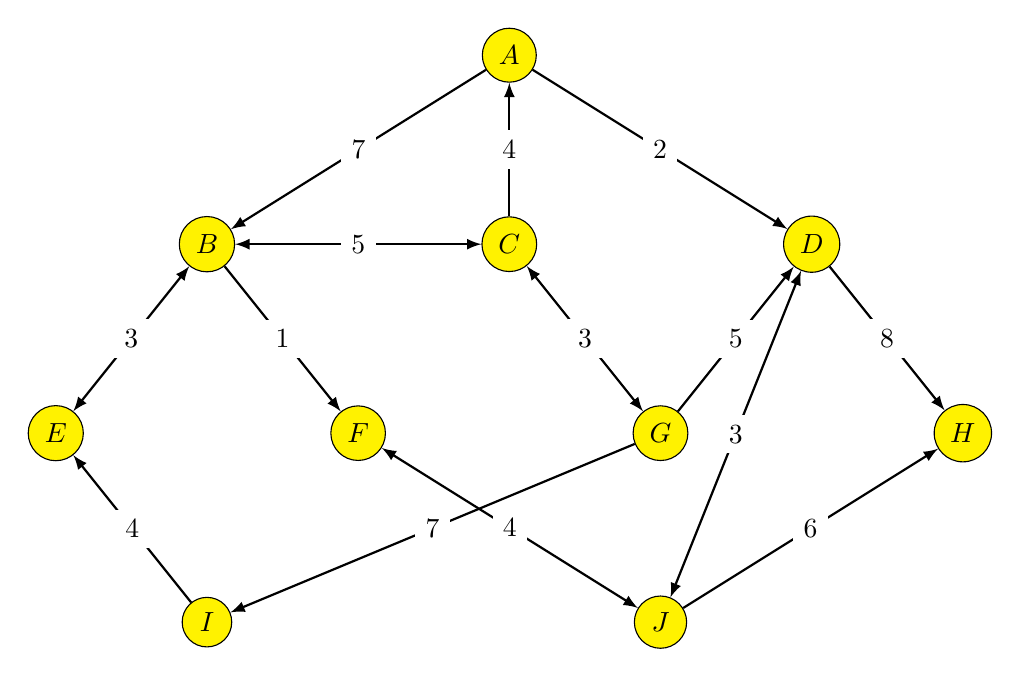
\begin{tikzpicture}[xscale=.8,yscale=.8]
% Styles (MODIFIABLES)
\tikzstyle{fleche}=[<->,>=latex,thick]
\tikzstyle{sfleche}=[->,>=latex,thick]
\tikzstyle{noeud}=[fill=yellow,circle,draw]
\tikzstyle{feuille}=[fill=orange,circle,draw]
\tikzstyle{etiquette}=[midway,fill=white,draw=white]
\tikzstyle{etiquette2}=[rectangle,fill=white,draw=white]
% Dimensions (MODIFIABLES)
\def\DistanceInterNiveaux{3}
\def\DistanceInterFeuilles{2}
% Dimensions calculées (NON MODIFIABLES)
\def\NiveauA{(-0)*\DistanceInterNiveaux}
\def\NiveauB{(-1)*\DistanceInterNiveaux}
\def\NiveauC{(-2)*\DistanceInterNiveaux}
\def\NiveauD{(-3)*\DistanceInterNiveaux}
\def\InterFeuilles{(1.2)*\DistanceInterFeuilles}
% Noeuds (MODIFIABLES : Styles et Coefficients d'InterFeuilles)
\node[noeud] (a) at ({(0)*\InterFeuilles},{\NiveauA}) {$A$};
\node[noeud] (b) at ({(-2)*\InterFeuilles},{\NiveauB}) {$B$};
\node[noeud] (c) at ({(0)*\InterFeuilles},{\NiveauB}) {$C$};
\node[noeud] (d) at ({(2)*\InterFeuilles},{\NiveauB}) {$D$};
\node[noeud] (e) at ({(-3)*\InterFeuilles},{\NiveauC}) {$E$};
\node[noeud] (f) at ({(-1)*\InterFeuilles},{\NiveauC}) {$F$};
\node[noeud] (g) at ({(1)*\InterFeuilles},{\NiveauC}) {$G$};
\node[noeud] (h) at ({(3)*\InterFeuilles},{\NiveauC}) {$H$};
\node[noeud] (i) at ({(-2)*\InterFeuilles},{\NiveauD}) {$I$};
\node[noeud] (j) at ({(1)*\InterFeuilles},{\NiveauD}) {$J$};
% Arcs (MODIFIABLES : Styles)
\draw[sfleche] (a)--(b) node[etiquette] {$7$};
\draw[sfleche] (c)--(a) node[etiquette] {$4$};
\draw[sfleche] (a)--(d) node[etiquette] {$2$};
\draw[fleche] (b)--(c) node[etiquette] {$5$};
\draw[fleche] (b)--(e) node[etiquette] {$3$};
\draw[sfleche] (b)--(f) node[etiquette] {$1$};
\draw[fleche] (c)--(g) node[etiquette] {$3$};
\draw[sfleche] (g)--(d) node[etiquette] {$5$};
\draw[sfleche] (d)--(h) node[etiquette] {$8$};
\draw[fleche] (d)--(j) node[etiquette] {$3$};
\draw[sfleche] (i)--(e) node[etiquette] {$4$};
\draw[sfleche] (g)--(i) node[etiquette] {$7$};
\draw[fleche] (f)--(j) node[etiquette] {$4$};
\draw[sfleche] (j)--(h) node[etiquette] {$6$};
\end{tikzpicture}
\end{center}
\item Implémenter en langage Python la fonction \code{parcours\_prof}.
\item L'arbre couvrant d'un graphe est un arbre qui a les mêmes sommets que le graphe et est obtenu en supprimant des arcs afin qu'il n'y ait aucun cycle et qu'il n'existe à chaque fois qu'un unique trajet entre deux sommets. 
\begin{enumerate}
\item Donner un arbre couvrant du graphe ci-dessus.
\item Expliquer comment on peut à partir du parcours en profondeur d'un graphe obtenir un arbre couvrant. 
\end{enumerate}
\end{enumerate}



\newpage
\section*{Exercice 3}
\emph{Cet exercice porte sur la programmation et utilise essentiellement de la Programmation Orientée Objet et les tableaux en langage Python.}\\
Un capteur est placé sur un moteur et commence à prendre des mesures de température à la mise en route de celui-ci.\\
Une mesure est stockée sous la forme d'un objet défini au moyen du constructeur suivant 
\begin{Python}
class mesure :
    def __init__(t,x):
        '''t : temps en secondes depuis la mise en route 
          x est la température mesurée (en deg. celsius)'''
        self.duree=t
        self.temp=x
\end{Python} 
\subsection*{\vskip - 7 mm Question 1}
\begin{enumerate}
\item Comment s'appellent \code{duree} et \code{temps} ?
\item Quelle instruction permet de créer une mesure \code{m} opérée 300 secondes après la mise en marche du moteur et indiquant une température de 275 degrés ? 
\item On a exécuté l'instructions \code{m1=mesure(730,200)}.\\
Que renvoie l'instruction \code{m1.duree} ? Que renvoie l'instruction \code{m1.temp>250} ? 
\item Pour plus de lisibilité, on veut pouvoir accéder au temps écoulé sous la forme d'un 3-uplet donnant les heures, les minutes et les secondes. 
\begin{enumerate}
\item A la main, convertir une durée de 7545 secondes en heures/minutes/secondes.
\item Compléter le code de la fonction suivante prévue à cet effet. \\
On rappelle que \code{//} donne le quotient de la division de deux entiers et \code{\%} donne le reste de la division de deux entiers. Ainsi, \code{10000//3600=2} et \code{10000\%3600=2800}
\begin{Python}
	def chrono(self):
		heures= #à compléter1
		secondes_restantes=#à compléter2
		minutes=#à compléter3
		secondes=#à compléter4
		return(heures,minutes,secondes)       
\end{Python} 
\item Comment s'appelle une fonction qui comme \code{chrono}, s'applique spécifiquement aux éléments d'une classe ?
\end{enumerate}
\end{enumerate}
On dispose maintenant de toute une série de mesures, mises dans un tableau Python \code{t}. 
\subsection*{\vskip - 7 mm Question 2}
On a exécuté les commandes suivantes : 
\begin{Python}
t=[]
t.append(mesure(0,17))
t.append(mesure(10,100))
t.append(mesure(20,210))
t.append(mesure(30,215))
t.append(mesure(40,217))
t.append(mesure(50,213))
\end{Python}
\begin{enumerate}
\item Que renvoient les appels 
\code{t[1]}  \hskip 1cm \code{t[2].duree} \hskip 1cm \code{t[4].temp} \hskip 1cm \code{t[6].temp}  ?
\item Au vu de ces données, décrire brièvement le protocole de mesure et les résultats observés
\item Compléter le code de la fonction \code{depassement} prenant comme paramètre \code{t} un tableau de mesures et une valeur \code{a} et renvoyant un tableau contenant les horaires (en seconde) auxquels la température mesurée a dépassé \code{a}.
\begin{Python}
# à compléter1
	val_dep=[]
	for mesu in t :
		if # à compléter2 
			val_dep.# à compléter3
	return(val_dep)
\end{Python}
\item Ecrire le code d'une fonction \code{temperature\_moy} prenant comme paramètre un tableau \code{t} de mesures et renvoyant la température moyenne relevée. 
\end{enumerate}
On s'intéresse maintenant aux problèmes de surchauffe du moteur et aux laps de temps pendant lesquels la température moteur dépasse une certaine valeur. On considère ainsi le code suivant : 
\begin{Python}
def depassement2(t,a):
	n=len(t)
	for k in range(0,n):
		if t[k].temp>a and t[k+1].temp>a and t[k+2].temp>a :
			return([t[k].duree,t[k+1].duree,t[k+2].duree)
	return('ok')
\end{Python}
En l'état, lorsqu'on l'exécute avec \code{t} un tableau de mesures et \code{a} un nombre, il donne parfois un message d'erreur du type \code{IndexError: list index out of range}
\subsection*{\vskip - 9 mm Question 3}
\begin{enumerate}
\item \begin{enumerate}
\item Justifier cette situation (existence et caractère non systématique de l'erreur).
\item Proposer une modification du programme permettant d'éviter cela.
\item Le programme ayant été corrigé, décrire simplement ce qu'il fait. En particulier, quand renvoie-t-il \code{'ok'} ?   
\end{enumerate}
\item \begin{enumerate}
\item Avec \code{len(t)=n}, combien de tests effectue au maximum la fonction \code{depassement2} ? 
\item Est-ce que tous ces tests sont utiles ? Pourquoi ?
\item On propose alors l'algorithme suivant, écrit en pseudo-code :
{\small \begin{Python}
Fonction depassement3(t,a)
n=longueur de t
c=0
k=0
Tant que c<3 et k<n
Si la température de la mesure t[k] est >a
Alors c=c+1
Sinon c=0
Fin Si
k=k+1
Fin Tant que       
Si c vaut 3 
Alors  # à compléter1
Sinon # à compléter2
Fin Si
\end{Python}}
Traduire en langage Python cet algorithme en complétant les deux lignes afin que \code{depassement2} et \code{depassement3} fournissent le même résultat.
\end{enumerate}
\end{enumerate}
%
%
%
%
\newpage
\section*{Exercice 4}
\emph{Cet exercice porte sur les bases de données relationnelles et sur le langage SQL.}


Vous êtes un nouvel ingénieur, embauché par la Compagnie des Trains Rapides (CTR) et votre mission consiste à définir les caractéristiques du réseau ferroviaire régional de cette compagnie, ainsi que des trains qui y circulent. Cela sera utilisé par exemple pour afficher sur les écrans d'information d'une gare les horaire des trains qui vont la desservir.


\begin{figure}[ht]
\centering
\includegraphics[width=12cm]{images/reseauFerre.JPG}
\caption{Schéma du réseau ferroviaire régional}
\end{figure}

%%%%%%%%%%%%%%%%%%%%%%%%%%%%%%%%%%%%%%%%%%%%%%%%%%%%%%%%%%%%%%%%%%%%%%%%%%
\subsection*{Question 1}
%%%%%%%%%%%%%%%%%%%%%%%%%%%%%%%%%%%%%%%%%%%%%%%%%%%%%%%%%%%%%%%%%%%%%%%%%%

Dans une première approche de votre mission, vous décidez de concevoir un tableau qui indique les gares desservies par chaque train. Le tableau a la forme suivante : 



\begin{center}
\begin{tabular}[c]{c|c|c|c|c}
IdTrain & NumLigne & Sens & NomGare & Horaire \\ \hline
AZ341 & 1 & + & B & 08:50 \\ \hline
AZ341 & 1 & + & C & 09:20 \\ \hline
DE666 & 2 & - & J & 13:20 \\ \hline
DE666 & 2 & - & D & 14:40 \\ \hline
... & ... & ... & ... & ... \\ \hline
\end{tabular}
\end{center}

\begin{enumerate}
 \item Citez trois problèmes qui peuvent se poser avec un tel tableau, lors de la création, l'utilisation ou la modification des données de ce tableau.
 \item Vous décidez rapidement qu'une bien meilleure approche consiste à stocker ces données à l'aide d'une base de données relationnelle. Citez trois exemples concrets (hors traffic ferroviaire) où des bases de données sont utilisées.
\end{enumerate}




%%%%%%%%%%%%%%%%%%%%%%%%%%%%%%%%%%%%%%%%%%%%%%%%%%%%%%%%%%%%%%%%%%%%%%%%%%
\subsection*{Question 2}
%%%%%%%%%%%%%%%%%%%%%%%%%%%%%%%%%%%%%%%%%%%%%%%%%%%%%%%%%%%%%%%%%%%%%%%%%%

La base de données que vous avez conçu est décrit par le schéma relationnel suivant :
\begin{itemize}
 \item \textsc{Gare} (\underline{Nom} (string), CorrespBus\footnote{Indique s'il y a une correspondance possible avec des bus.} (boolean))
 \item \textsc{Ligne} (\underline{Num} (integer), \emph{NomGareDebut} (string))
 \item \textsc{Train} (\underline{Id} (string), \emph{NumLigne} (integer), Sens (string))
 \item \textsc{Reseau} (\underline{\emph{NomGare}} (string), \underline{\emph{NumLigne}} (integer), PtKilometriq\footnote{Indique la distance de la gare à la gare de début de ligne, en km, dans le sens '+'.} (integer))
 \item \textsc{Desserte} (\underline{Id} (integer), \emph{NomGare} (string), \emph{IdTrain} (string), Horaire\footnote{Le format de l'horaire est HH:MM} (time))
\end{itemize}

\begin{enumerate}
 \item Quel nom donne-t-on aux différents termes tels que \verb'Id', \verb'CorrespBus', ou \verb'Horaire' ? Quel nom donne-t-on à une ligne présente dans une relation ?
 \item D'après vous, que représentent les termes soulignés ? Quel rôle joue ce type de terme dans une relation ?
 \item D'après vous, que représentent les termes en italique ?
\end{enumerate}


%%%%%%%%%%%%%%%%%%%%%%%%%%%%%%%%%%%%%%%%%%%%%%%%%%%%%%%%%%%%%%%%%%%%%%%%%%
\subsection*{Question 3}
%%%%%%%%%%%%%%%%%%%%%%%%%%%%%%%%%%%%%%%%%%%%%%%%%%%%%%%%%%%%%%%%%%%%%%%%%%

La base de données est supposée déjà partiellement remplie. Mais il faut régulièrement la mettre à jour, suite à certains évènements.

\begin{enumerate}
 \item Un nouveau train va être mis en circulation sur la ligne 1, dans le sens '-'. Son identifiant est 'PP1234'. Ce train part à 08:00 de la gare 'I' et arrive à 10:00 à la gare 'G', en desservant à 09:00 la gare 'D'. Ecrire, à l'aide de la commande \verb'INSERT INTO', les commandes SQL ajoutant toutes ces informations dans la BDD. On rappelle que la syntaxe d'utilisation de cette commande est : 
 \begin{verbatim}
  INSERT INTO nom_de_la_table VALUES (valeur_1, valeur_2, ...)
 \end{verbatim}
 A noter que l'identifiant de desserte est automatiquement incrémenté lors de l'ajout d'une nouvelle desserte et n'a donc pas besoin d'être précisé.
 \item Le train 'FX0102', desservant toutes les gares de la ligne 3 dans le sens '+', ne peut démarrer à cause d'un problème technique. Vous décidez de le supprimer à l'aide de la commande SQL suivante : 
 \begin{verbatim}
  DELETE FROM Train WHERE Id = 'FX0102'
 \end{verbatim}
 Mais le Système de Gestion de Bases de Données (SGBD) refuse d'exécuter cette commande et renvoie un message d'erreur (alors que la syntaxe est bien correcte). Expliquez pourquoi ? Proposez une solution à ce problème.
 \item Vous apprenez que le train 'ZE6321' de la ligne 2 en sens '+' doit ralentir après la gare 'J' et arrivera à 13:10 à la gare 'E', au lieu de 12:50. Ecrire, à l'aide de la commande \verb'UPDATE', la ou les commandes SQL mettant à jour ces informations dans la BDD. On rappelle que la syntaxe d'utilisation de cette commande est : 
 \begin{verbatim}
  UPDATE nom_de_la_table 
  SET nom_de_col1 = valeur1, nom_de_col2 = valeur2, ... 
  WHERE condition
 \end{verbatim}
\end{enumerate}



%%%%%%%%%%%%%%%%%%%%%%%%%%%%%%%%%%%%%%%%%%%%%%%%%%%%%%%%%%%%%%%%%%%%%%%%%%
\subsection*{Question 4}
%%%%%%%%%%%%%%%%%%%%%%%%%%%%%%%%%%%%%%%%%%%%%%%%%%%%%%%%%%%%%%%%%%%%%%%%%%

Dans cette question, vous devez écrire des requêtes SQL permettant de renvoyer des informations exigées, à l'aide des seules commandes SQL suivantes : \verb'WHERE', \verb'MAX', \verb'DISTINCT', \verb'COUNT', \verb'AS', \verb'FROM', \verb'SELECT', \verb'JOIN', \verb'ON', \verb'ORDER BY', \verb'LIMIT', \verb'SUM', \verb'DESC', \verb'OFFSET', \verb'MIN'. Vous pouvez également effectuer des sous-requêtes ou des requêtes imbriquées, si besoin est.

\begin{enumerate}
 \item Afficher toute la table \textsc{Train}.
 \item Afficher les noms de toutes les gares du réseau régional, avec un tri selon l'ordre alphabétique croissant.
 \item Afficher le nombre de toutes les gares qui possèdent une correspondance avec un réseau de bus.
 \item Afficher le nom et la position kilométrique de toutes les gares de la ligne 3, avec un tri selon l'ordre croissant des positions kilométriques.
 \item Afficher, sans répétition, le numéro des lignes qui passent par la gare 'J'.
 \item Afficher la longueur totale de la ligne 1.
 \item Afficher le nom de tous les trains qui desservent la gare 'D' selon le sens '+'. Attention, on ne veut pas de répétition de noms de train (ce qui peut avoir lieu si un train passe plusieurs fois par cette gare dans ce sens, au cours de la journée).
 \item Afficher, sans répétition de train, le nombre de trains qui circulent sur la ligne 3, après 20:00.
\end{enumerate}
%
%
%
%
\newpage
\section*{Exercice 5}
\emph{Cet exercice comporte trois parties indépendantes portant sur les commandes Linux et les protocoles réseaux.}
\subsection*{Partie 1 : Commandes Linux}
On rappelle les commandes suivantes : \medskip\\
\begin{tabular}{|l|l|}\hline
Commande & Description \\ \hline
\code{pwd} & Affiche le nom du répertoire courant \\ \hline
\code{ls} & Liste le contenu du répertoire courant \\ \hline
\code{cd}  & Change de répertoire courant  \\ \hline
\code{mkdir}& Crée un nouveau répertoire  \\ \hline
\code{cp}& Crée une copie d'un fichier ou d'un répertoire \\ \hline
\code{rm}& Supprime un répertoire ou un fichier \\ \hline
\code{touch}& Crée un fichier (entre autres choses) \\ \hline\hline
\code{*.*}& Désigne le contenu complet d'un répertoire. \\ \hline
\end{tabular}\medskip\\
A noter que ces commandes s'utilisent avec des attributs, en particuliers des noms de répertoires/fichiers et des chemins d'accès. On distingue ainsi : 
\begin{itemize}
\item les chemins absolus, donnés à partir de la racine, commençant par $/$
\item les chemins relatifs, donnés à partir de la position actuelle, commençant par le nom du premier répertoire.
\end{itemize}
Ainsi, si on dispose d'un système de fichier avec l'arborescence suivante, 
\begin{figure}[ht]
\centering
\includegraphics[width=14cm]{images/arbre2.JPG}
\caption{Arborescence \label{arbo}}
\end{figure}
\begin{itemize}
\item En partant de la racine \code{C}, \code{cd /rep1/rep4/rep7} et \code{cd rep1/rep4/rep7}  mènent dans \code{rep7}. Comme on démarre de la racine, il n'y a pas de différence entre chemin relatif et absolu.
\item Une fois dans \code{rep7}, \code{cd ../../rep6} mène dans \code{rep6} (le \code{..} signifie reculer d'un rang dans l'arborescence).
\item Une fois dans \code{rep6}, la commande \code{cd /rep2} mène directement dans \code{rep2}. Commençant par un \code{/}, c'est un chemin absolu démarrant à la racine.  
\item De même, \code{mkdir /rep2/rep8} créera un répertoire \code{rep8} à l'intérieur de \code{rep2}, peu importe l'endroit depuis lequel la commande est lancée.
\item Tandis que si on est dans \code{rep7}, 
\begin{itemize}
\item \code{touch ../../essai.txt} créera un fichier \code{essai.txt} à l'intérieur de \code{rep1}
\item \code{mkdir rep9} créera un répertoire \code{rep9} dans \code{rep7}
\item \code{mkdir /rep10} créera un répertoire \code{rep10} directement à la racine
\end{itemize}
\end{itemize}
%%%%%%%%%%%%%%%%%%%%%%%%%%%%%%%%%%%%%%%%%%%%%%%%%%%%%%%%%%%%%%%%%%%%%%%%%%
\subsection*{Question 1}
%%%%%%%%%%%%%%%%%%%%%%%%%%%%%%%%%%%%%%%%%%%%%%%%%%%%%%%%%%%%%%%%%%%%%%%%%%
\begin{enumerate}
\item On suppose que :
\begin{itemize}
\item Tous les dossiers et fichiers de la Figure \ref{arbo} ont été crées, sauf la partie encadrée.
\item On vient de taper la commande \code{pwd} dans le shell et on a obtenu comme réponse \code{/rep3}.
\end{itemize}
\vskip 3mm
Donner un jeu de commandes permettant de créer les dossiers et les fichiers de la partie encadrée.
\item On suppose maintenant que tous les dossiers et fichiers de la Figure \ref{arbo} ont été créées.\\
On entre alors les commandes suivantes en console : 
\begin{Python}
rm /rep2
cd /rep1/rep4/rep7
cp *.* /rep3
cp ../../rep6/*.*  /rep3
cd ..
cd ..
rm *.*
\end{Python}
Dessiner, en justifiant brièvement, l'arborescence résultant de ces opérations. 
\end{enumerate}
\subsection*{Partie 2 : Protocole RIP}
On considère le réseau suivant (chaque routeur est repéré par une lettre) :
\begin{center}
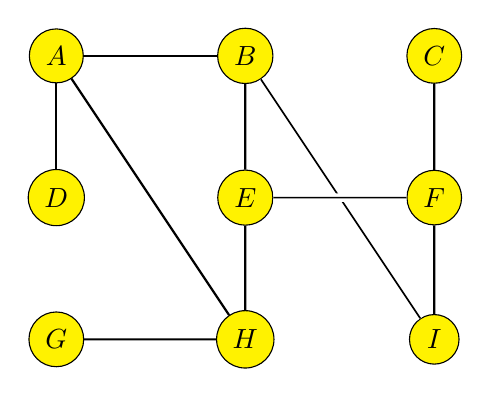
\begin{tikzpicture}[xscale=0.8,yscale=0.8]
% Styles (MODIFIABLES)
\tikzstyle{fleche}=[-,>=latex,thick]
\tikzstyle{noeud}=[fill=yellow,circle,draw]
\tikzstyle{feuille}=[fill=orange,circle,draw]
% Dimensions (MODIFIABLES)
\def\DistanceInterNiveaux{3}
\def\DistanceInterFeuilles{2}
% Dimensions calculées (NON MODIFIABLES)
\def\NiveauA{(-0)*\DistanceInterNiveaux}
\def\NiveauB{(-.75)*\DistanceInterNiveaux}
\def\NiveauC{(-1.5)*\DistanceInterNiveaux}
\def\InterFeuilles{(.75)*\DistanceInterFeuilles}
% Noeuds (MODIFIABLES : Styles et Coefficients d'InterFeuilles)
\node[noeud] (Ra) at ({(0)*\InterFeuilles},{\NiveauA}) {$A$};
\node[noeud] (Rb) at ({(2)*\InterFeuilles},{\NiveauA}) {$B$};
\node[noeud] (Rc) at ({(4)*\InterFeuilles},{\NiveauA}) {$C$};
\node[noeud] (Rd) at ({(0)*\InterFeuilles},{\NiveauB}) {$D$};
\node[noeud] (Re) at ({(2)*\InterFeuilles},{\NiveauB}) {$E$};
\node[noeud] (Rf) at ({(4)*\InterFeuilles},{\NiveauB}) {$F$};
\node[noeud] (Rg) at ({(0)*\InterFeuilles},{\NiveauC}) {$G$};
\node[noeud] (Rh) at ({(2)*\InterFeuilles},{\NiveauC}) {$H$};
\node[noeud] (Ri) at ({(4)*\InterFeuilles},{\NiveauC}) {$I$};
% Arcs (MODIFIABLES : Styles)
\draw[fleche] (Ra)--(Rb);
\draw[fleche] (Ra)--(Rd);
\draw[fleche] (Ra)--(Rh);
\draw[fleche] (Rb)--(Re);
\draw[fleche,draw=white,double=black,very thick] (Rb)--(Ri);
\draw[fleche] (Rc)--(Rf);
\draw[fleche,draw=white,double=black,very thick] (Re)--(Rf);
\draw[fleche] (Re)--(Rh);
\draw[fleche] (Rf)--(Ri);
\draw[fleche] (Rg)--(Rh);
\end{tikzpicture}
\end{center}
Pour les questions suivantes, on se place dans le cadre du protocole RIP.\\
Pour départager des chemins de même longueur, on considère qu'à chaque fois que cela était possible, les connexions ont été établies dans l'ordre alphabétique. \\
Ainsi, la liaison entre \code{A} et \code{B} a été créée avant celle entre \code{A} et \code{D},...\\
De plus, un chemin entre deux routeurs est remplacé par un autre chemin uniquement si le nouveau chemin est strictement plus court.
\subsection*{Question 2}
\begin{enumerate}
    \item Quel est le chemin de A vers F ?
    \item Recopier sur votre copie et compléter la table de routage du routeur B (sur le modèle de la table du {\bf 3)}:
    \begin{center}
        \begin{tabular}{|c|c|c|}\hline
            Destination&Routeur suivant&Distance\\ \hline
            $\vdots$ &$\vdots$&$\vdots$\\ \hline
            
        \end{tabular}
    \end{center}
    \item Une liaison directe a été ajoutée entre deux routeurs.
    La nouvelle table de routage du routeur F est alors :
    \begin{center}
        \begin{tabular}{|c|c|c|}\hline
            Destination&Routeur suivant&Distance\\ \hline
            A&E &3 \\ \hline
            B&E &2 \\ \hline
            C&C &1 \\ \hline
            D&I &2 \\ \hline
            E&E &1 \\ \hline
            G&E &3 \\ \hline
            H&E &2 \\ \hline
            I&I &1 \\ \hline
        \end{tabular}
    \end{center}
    Entre quels routeurs la liaison a-t-elle été ajoutée ? Justifier brièvement.
    
\end{enumerate}
\subsection*{Partie 3 : Protocole OSPF}
On considère le réseau suivant (chaque routeur est repéré par une lettre) :
\begin{multicols}{2}
\begin{center}
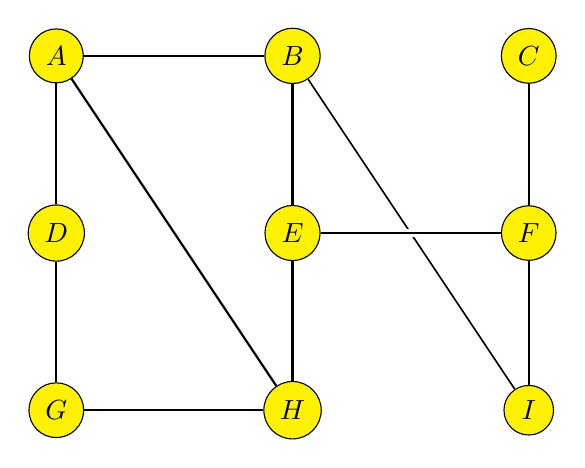
\begin{tikzpicture}[xscale=1,yscale=1]
% Styles (MODIFIABLES)
\tikzstyle{fleche}=[-,>=latex,thick]
\tikzstyle{noeud}=[fill=yellow,circle,draw]
\tikzstyle{feuille}=[fill=orange,circle,draw]
% Dimensions (MODIFIABLES)
\def\DistanceInterNiveaux{3}
\def\DistanceInterFeuilles{2}
% Dimensions calculées (NON MODIFIABLES)
\def\NiveauA{(-0)*\DistanceInterNiveaux}
\def\NiveauB{(-.75)*\DistanceInterNiveaux}
\def\NiveauC{(-1.5)*\DistanceInterNiveaux}
\def\InterFeuilles{(.75)*\DistanceInterFeuilles}
% Noeuds (MODIFIABLES : Styles et Coefficients d'InterFeuilles)
\node[noeud] (Ra) at ({(0)*\InterFeuilles},{\NiveauA}) {$A$};
\node[noeud] (Rb) at ({(2)*\InterFeuilles},{\NiveauA}) {$B$};
\node[noeud] (Rc) at ({(4)*\InterFeuilles},{\NiveauA}) {$C$};
\node[noeud] (Rd) at ({(0)*\InterFeuilles},{\NiveauB}) {$D$};
\node[noeud] (Re) at ({(2)*\InterFeuilles},{\NiveauB}) {$E$};
\node[noeud] (Rf) at ({(4)*\InterFeuilles},{\NiveauB}) {$F$};
\node[noeud] (Rg) at ({(0)*\InterFeuilles},{\NiveauC}) {$G$};
\node[noeud] (Rh) at ({(2)*\InterFeuilles},{\NiveauC}) {$H$};
\node[noeud] (Ri) at ({(4)*\InterFeuilles},{\NiveauC}) {$I$};
% Arcs (MODIFIABLES : Styles)
\draw[fleche] (Ra)--(Rb);
\draw[fleche] (Ra)--(Rd);
\draw[fleche] (Ra)--(Rh);
\draw[fleche] (Rb)--(Re);
\draw[fleche] (Rd)--(Rg);
\draw[fleche,draw=white,double=black,very thick] (Rb)--(Ri);
\draw[fleche] (Rc)--(Rf);
\draw[fleche,draw=white,double=black,very thick] (Re)--(Rf);
\draw[fleche] (Re)--(Rh);
\draw[fleche] (Rf)--(Ri);
\draw[fleche] (Rg)--(Rh);
\end{tikzpicture}
\end{center}

\begin{tabular}{|l|l|l|}\hline
    Liaison& Type   & Débit\\\hline
    A$\leftrightarrow$B&Bluetooth&5 Mbit/s \\\hline
    A$\leftrightarrow$D&Ethernet&20 Mbit/s \\\hline
    A$\leftrightarrow$H&Fibre&1 Gbit/s \\\hline
    B$\leftrightarrow$E&Bluetooth&5 Mbit/s\\\hline
    B$\leftrightarrow$I&Fast Ethernet&100 Mbit/s\\\hline
    C$\leftrightarrow$F&Fibre&1 Gbit/s \\\hline
   D$\leftrightarrow$G&Fast Ethernet&100 Mbit/s  \\\hline
    E$\leftrightarrow$F&Wi-Fi&200 Mbit/s \\\hline
	E$\leftrightarrow$H&Fast Ethernet&100 Mbit/s \\\hline
    F$\leftrightarrow$I&Ethernet&20 Mbit/s \\\hline
    G$\leftrightarrow$H&Ethernet&10 Mbit/s \\\hline
    \end{tabular}
\end{multicols}
Pour les questions suivantes, on se place dans le cadre du protocole OSPF.
On rappelle que pour ce protocole, le coût d'une liaison est 
$\text{coût}=\frac{10^8}{d}$ où $d$ est la bande passante en $bit/s$.
\subsection*{Question 3}
\begin{enumerate}
    \item Quel est le coût des liaisons AB et AH ? Détailler les calculs.
    \item Sans autres justifications, recopier sur votre copie le graphe et donner la pondération de chacun des arcs. 
    \item Quel est le coût total du chemin D-A-B-E ?
    \item En justifiant brièvement, quel est le chemin le moins coûteux allant de G à B ?
\end{enumerate}

\end{document}

